%----------------------------------------------------------------------------------------
%	PACKAGES AND THEMES
%----------------------------------------------------------------------------------------
\documentclass[aspectratio=169,xcolor=dvipsnames]{beamer}
\usetheme{Simple}
\usepackage{hyperref}
\usepackage{hyperref}
\usepackage{graphicx} % Allows including images
\usepackage{booktabs} % Allows the use of \toprule, \midrule and \bottomrule in tables
\usepackage{graphicx}
%----------------------------------------------------------------------------------------
%	TITLE PAGE
%----------------------------------------------------------------------------------------

% The title
\title[short title]{Project Proposal}
\subtitle{Semi-supervised Sequence Learning}

\author[Sanjay K V] {Sabiha Sultana\inst{1}, Piyakorn Munegan\inst{2},\\ Sanjay Kanakkot Viswanathan\inst{3},\break Mohammed Rizwan Amanullah\inst{4}}
\institute[NTU] % Your institution may be shorthand to save space
{
    % Your institution for the title page
    Department of Computing, \\
    Macquarie University 
    \vskip 3pt
}
\date{\today} % Date, can be changed to a custom date


%----------------------------------------------------------------------------------------
%	PRESENTATION SLIDES
%----------------------------------------------------------------------------------------

\begin{document}

\begin{frame}
    % Print the title page as the first slide
    \titlepage
\end{frame}

\begin{frame}{Overview}
    % Throughout your presentation, if you choose to use \section{} and \subsection{} commands, these will automatically be printed on this slide as an overview of your presentation
    \tableofcontents
%------------------------------------------------
%Overview
%------------------------------------------------
\begin{itemize}
        \item In this paper, they have introduced two approaches, to use unlabelled data to improve sequence learning with Recurrent network \break
        - \textbf{First approach (LM-LSTM)} Language modelling. Predict what comes next in a sequence \break
        - \textbf{Second approach (SA-LSTM)} Sequence auto encoder.  Reads input sequence into vectors and predict the input sequence again.
    \end{itemize}

 %Adding picture
  \begin{figure}
  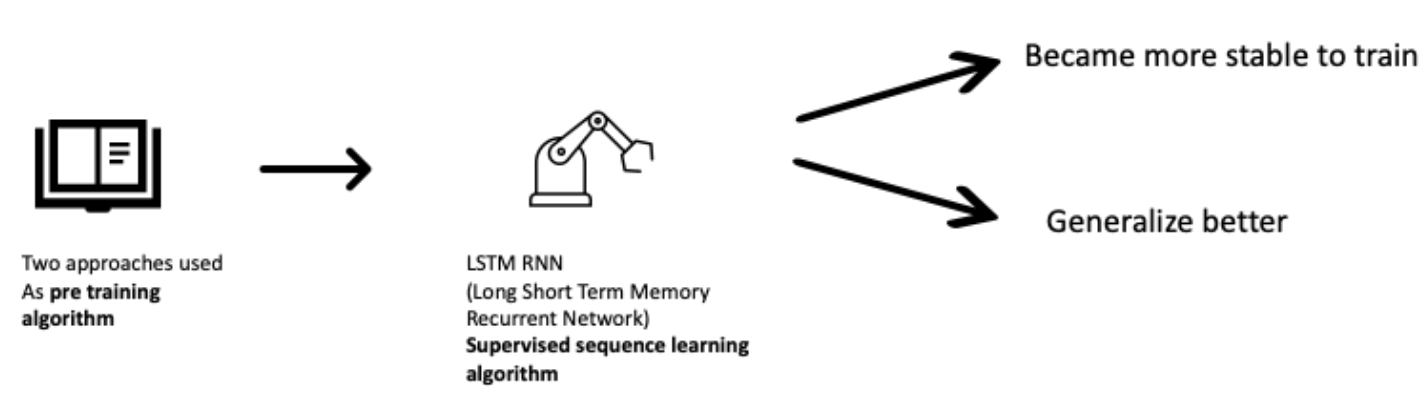
\includegraphics[width=250]{Project Proposal Presentation.png}
\end{figure}
%------------------------------------------------
\textbf{Claims}
        - Pre-trained LSTM Results in strong performance in many classification tasks.\break
        - Pre-trained LSTM performs better than LSTM initialized randomly. \break
        - It is possible to use unsupervised learning with more unlabelled data to improve supervised learning.
 
  
\end{frame}
%------------------------------------------------
%justification of original work
%------------------------------------------------

\begin{frame}{Justification for Project Basis}
    \begin{itemize}
        \item In Google Scholar this research paper has been cited by 989 people.
        \item Research paper has been published at Neural Information Processing Systems \break  (NIPS 2015), CORE ranking A*. \href{http://https://arxiv.org/pdf/1511.01432v1.pdf}{Link to Paper}. 
        \item  Code has been made available on the official Tensor Flow GitHub Page.
        \item  It covers in the area of Natural Language Processing(NPL); Recurrent Neural Networks (RNNs), Long Short-Term Memory recurrent networks (LSTM RNNs) and Sequence Autoencoder Long Short-Term Memory recurrent networks (SA-LSTMs).
    \end{itemize}
\end{frame}

%------------------------------------------------

\begin{frame}{Replication of original work}
    In this paper there were 4 data set \alert{IMDb, Rotten Tomatoes, DBpedia, 20 newsgroups} and different technique used for the same. 
    
 
   
  \begin{table}[h!]
  \begin{center}
    \caption{A summary of the error rates of SA-LSTMs and previous best reported results.}
    \label{tab:table1}
    \begin{tabular}{l|c|r} % <-- Alignments: 1st column left, 2nd middle and 3rd right, with vertical lines in between
      \hline
      \textbf{Dataset } & \textbf{SA-LSTM} & \textbf{Previous best results}\\
      
      \hline
      IMDB & 7.24\% & 7.42\% \\
      Rotten Tomatoes & 16.7\% & 18.5\% \\
      20 Newsgroups & 15.6\% & 17.1\% \\
      DBpedia & 1.19\% & 1.74\% \\
      \hline
     
    \end{tabular}
  \end{center}
\end{table}
%------------------------------------------------
   
\end{frame}

%------------------------------------------------
%justification of original work
%------------------------------------------------

\begin{frame}{New Data Generation}
    \begin{columns}[c] % The "c" option specifies centered vertical alignment while the "t" option is used for top vertical alignment

        \column{.45\textwidth} % Left column and width
        \textbf{The Process}
        \begin{enumerate}
            \item Creating Python Script
            \item Scrapping the data 
            \item Eg :Using "BeautifulSoup" python package
        \end{enumerate}

        \column{.5\textwidth} % Right column and width
         Using Python Script we will scrap the recent reviews & replicate the data similar way with other  Wikipedia, Rotten Tomatoes, GMB, DBpedia, Apple Reviews data set etc.

    \end{columns}
\end{frame}


%----------------------------------------------------------------------------------------

\begin{frame}
    \Huge{\centerline{The End}}
\end{frame}

%----------------------------------------------------------------------------------------

\end{document}